\section{转录组学}

\subsubsection{组学概述}
\begin{frame}
  \frametitle{转录组学 | \textcolor{red}{组学}}
  \begin{figure}
    \centering
    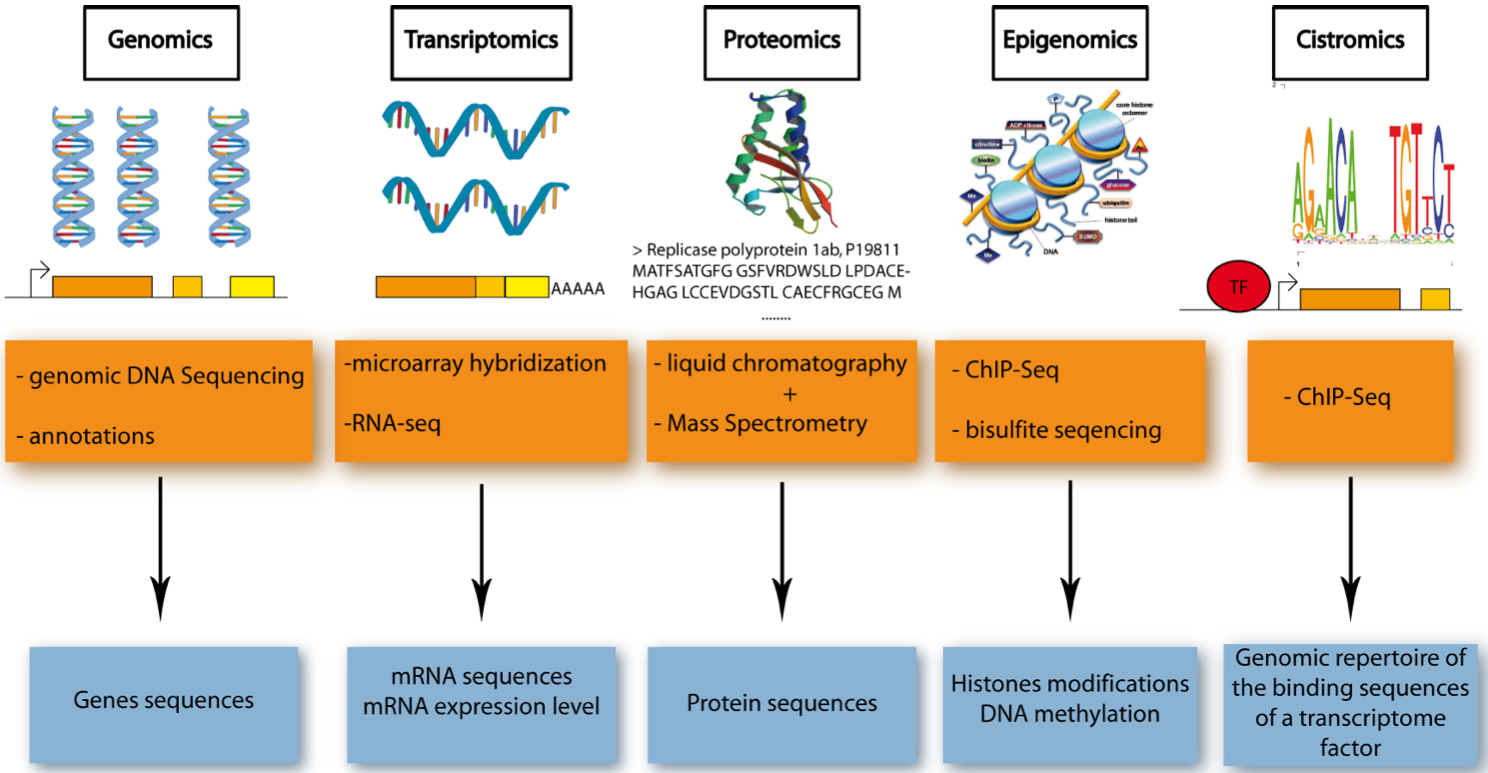
\includegraphics[width=0.95\textwidth]{c3_transcriptome/omics_03.png}
  \end{figure}
\end{frame}

\begin{frame}
  \frametitle{转录组学 | 组学}
  \begin{figure}
    \centering
    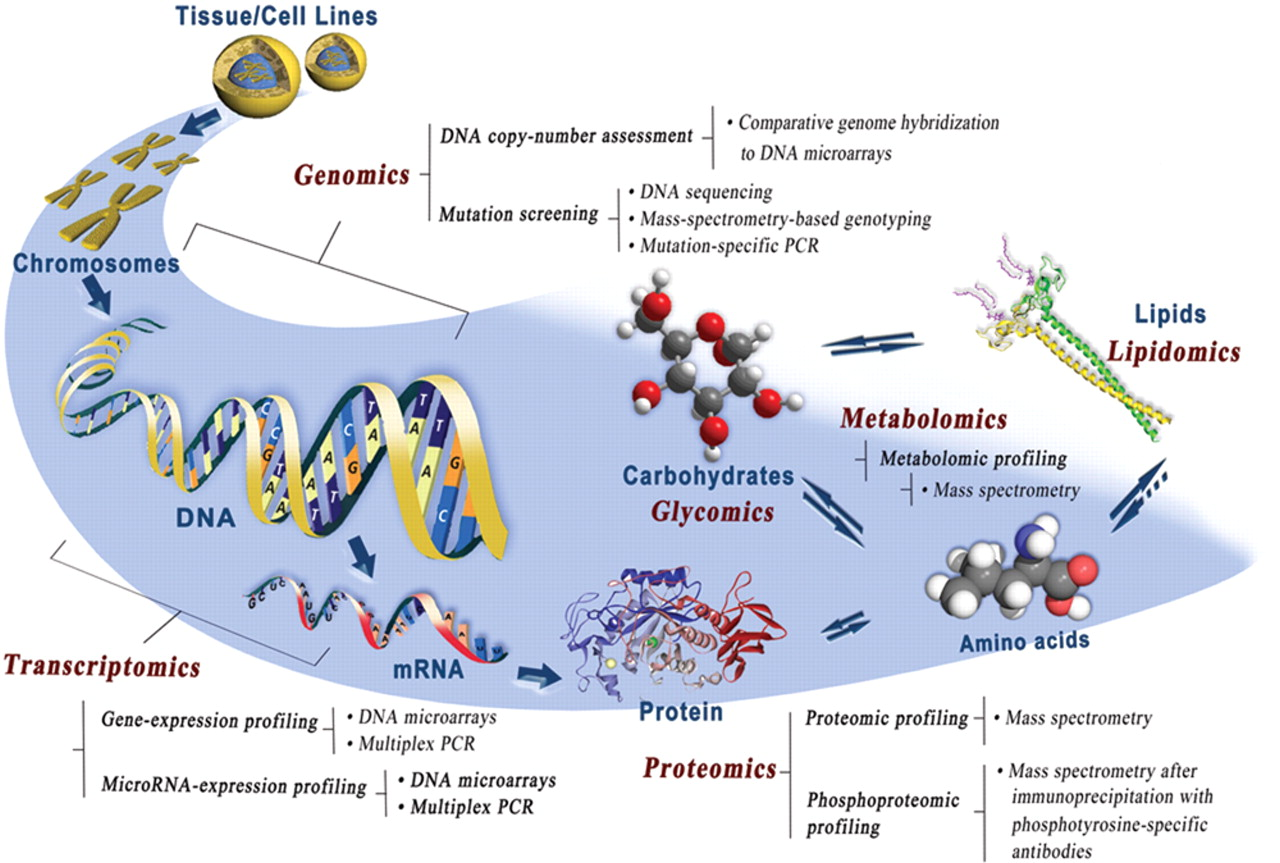
\includegraphics[width=0.9\textwidth]{c3_transcriptome/omics_04.jpg}
  \end{figure}
\end{frame}

\subsubsection{转录组学}
\begin{frame}
  \frametitle{转录组学 | 概述 | 转录组}
  \begin{block}{\textcolor{red}{转录组}}
转录组(transcriptome),也称为“转录物组”,广义上指在相同环境(或生理条件)下的在一个细胞、或一群细胞中所能转录出的所有RNA的总和,包括信使RNA(mRNA)、核糖体RNA(rRNA)、转运RNA(tRNA)及非编码RNA;狭义上则指细胞所能转录出的所有信使RNA(mRNA)。
  \end{block}
  \begin{figure}
    \centering
    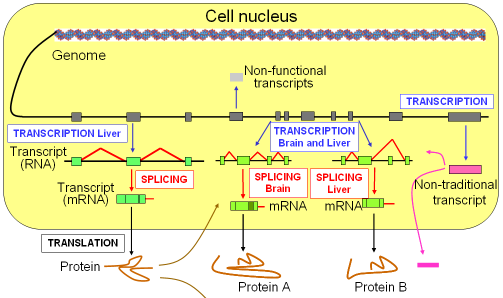
\includegraphics[width=0.65\textwidth]{c3_transcriptome/general_trans_01.png}
  \end{figure}
\end{frame}

\begin{frame}
  \frametitle{转录组学 | 概述 | 转录组学}
  \begin{block}{\textcolor{red}{转录组学}}
转录组学(或“转录物组学”,transcriptomics)是分子生物学的分支,负责研究在单个细胞或一个细胞群的特定细胞类型内所生产的mRNA分子。\\
    \vspace{0.5em}
    转录组学是对转录水平上发生的事件及其相互关系和意义进行整体研究的一门学科。
  \end{block}
  \pause
  \begin{block}{问题}
    \begin{itemize}
      \item 一个细胞、组织或生物体的全部RNA集合体中包括多少种RNA,各种RNA的数量有多少?
      \item 在不同发育时期和不同外界环境作用下RNA集合体会出现怎样的变化?
      \item 在细胞中转录是怎样被调节的?
      \item ……
    \end{itemize}
  \end{block}
\end{frame}

\begin{frame}
  \frametitle{转录组学 | 概述 | 转录组学 | 研究内容}
  \begin{figure}
    \centering
    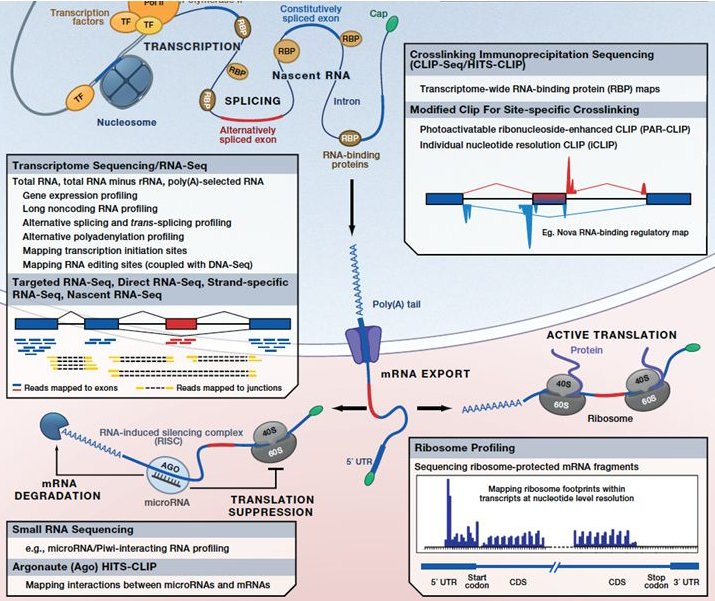
\includegraphics[width=0.75\textwidth]{c3_transcriptome/general_trans_content_01.jpg}
  \end{figure}
\end{frame}

\subsubsection{研究方法}
\begin{frame}
  \frametitle{转录组学 | 研究方法 | 概述}
  \begin{figure}
    \centering
    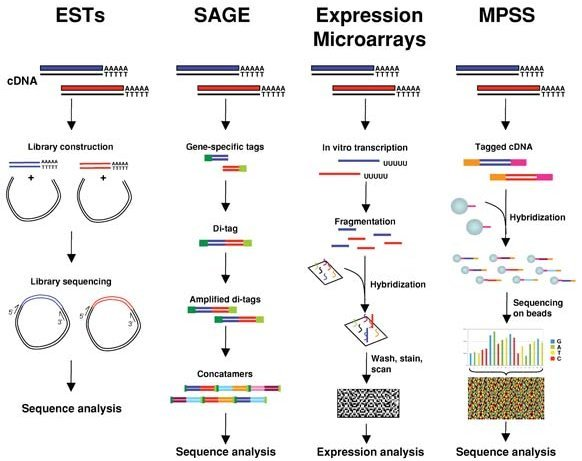
\includegraphics[width=0.8\textwidth]{c3_transcriptome/trans_method_01.jpg}
  \end{figure}
\end{frame}

\begin{frame}
  \frametitle{转录组学 | 研究方法 | 概述}
  \begin{figure}
    \centering
    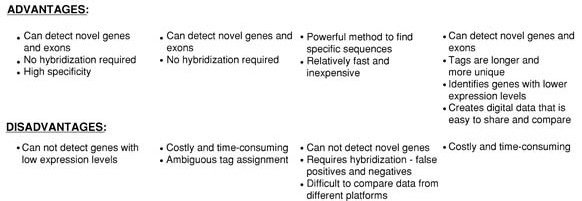
\includegraphics[width=0.9\textwidth]{c3_transcriptome/trans_method_02.jpg}
  \end{figure}
\end{frame}

\begin{frame}
  \frametitle{转录组学 | 研究方法 | 概述}
  \begin{figure}
    \centering
    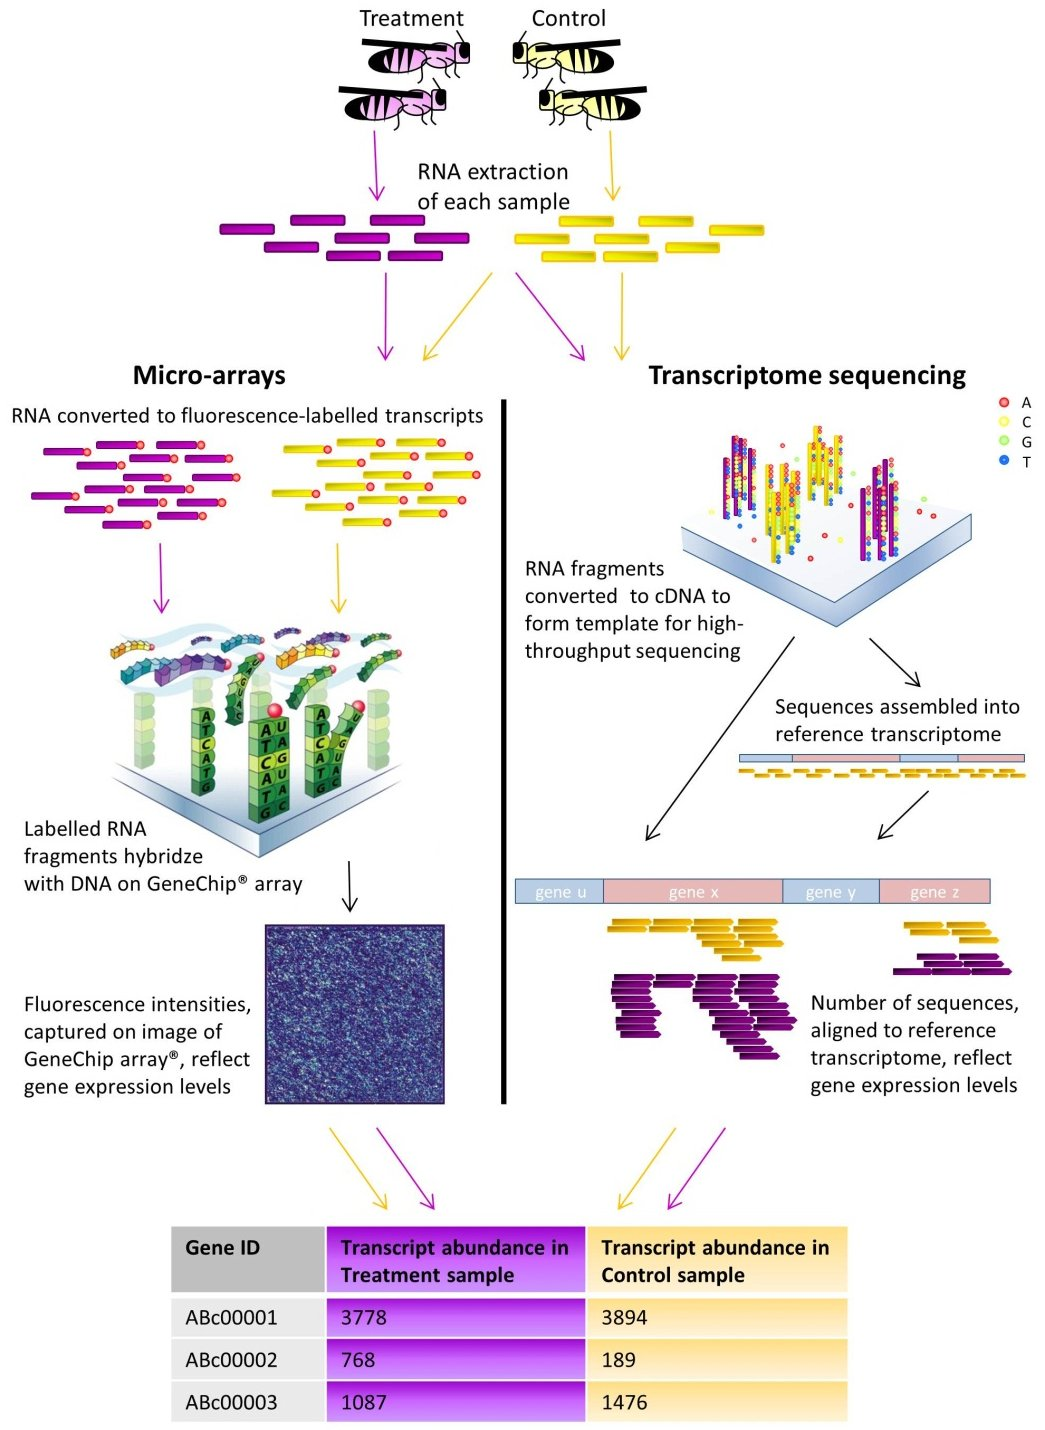
\includegraphics[width=0.5\textwidth]{c3_transcriptome/trans_method_03.jpg}
  \end{figure}
\end{frame}

\begin{frame}
  \frametitle{转录组学 | 研究方法 | \textcolor{red}{Microarray vs. RNA-Seq}}
  \begin{figure}
    \centering
    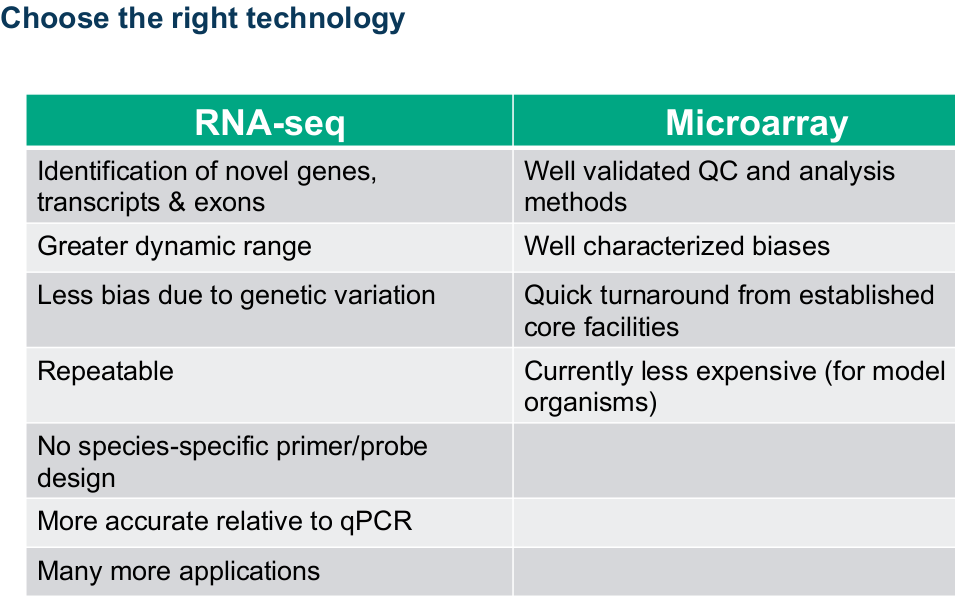
\includegraphics[width=0.9\textwidth]{c3_transcriptome/method_array_seq_01.png}
  \end{figure}
\end{frame}

